\chapter{运行与测试} 
%\pagenumbering{arabic} % 阿拉伯数字页码
本工程的性质是简易操作系统内核(当然还不算很完整),与Windows
下的exe文件性质不同,因此有必要谈谈如何运行测试.这里谈两种,
一是在物理裸机上运行,二是利用虚拟机完成运行测试;从学习原理的目的
出发,折腾前一种没有多大必要,而且可能有格式化硬盘的危险,还是推荐后一种方法.

\section{物理裸机}
\subsection{GRUB}
安装GRUB2到U盘的方法已经讲过,这里主要就是把编译后生成的build目录下的grub.cfg
和kernel.bin拷贝到U盘的相应位置即可.可能没有权限,用sudo cp的办法可以实现.
这里一定要注意路径的问题,路径放得不对就没有效果了.

如图~\ref{grub_folder01}~及图~\ref{grub_folder02}~所示.		

\begin{figure}[!htbp]
		\centering	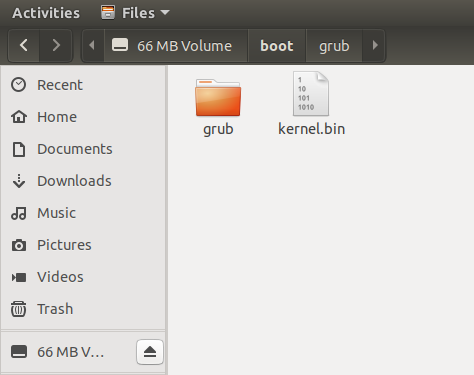
\includegraphics[width=14cm]{pic/assets/testcase/grub_folder01}
		\caption{U盘目录01}	\label{grub_folder01}	\end{figure}



\begin{figure}[!htbp]
		\centering	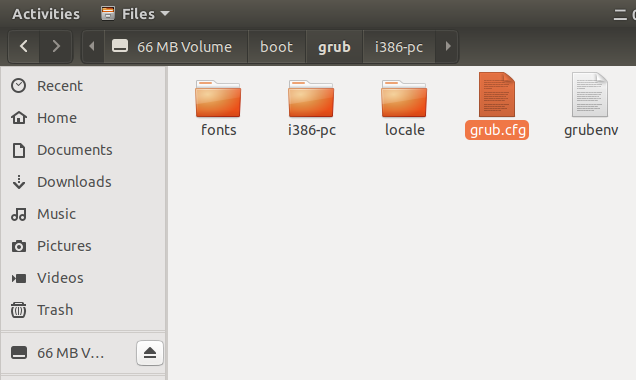
\includegraphics[width=14cm]{pic/assets/testcase/grub_folder02}
		\caption{U盘目录02}	\label{grub_folder02}	\end{figure}

U盘拷贝完的结构如图~\ref{grub_folder01}~所示.

\begin{figure}[!htbp]
		\centering	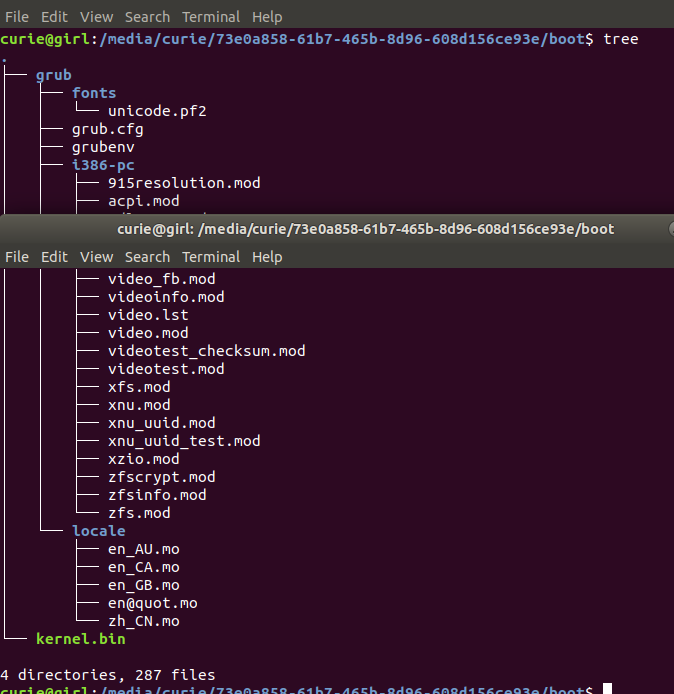
\includegraphics[width=14cm]{pic/assets/testcase/grub_tree}
        \caption{U盘目录02}	\label{grub_tree}	\end{figure}
        
好,接下来和U盘装系统的步骤应该差不多了,不过值得注意的是,为了建立文件系统,第一次进系统时,
我将把格式化整个物理硬盘,要注意数据的备份,比较危险.因为这个原因,在内核写到文件系统之前,
均在裸机上进行过验证性测试,之后因为要格式化硬盘的原因,只在qemu上测试了.把生成的
RiOS-i386.iso镜像通过其他途径烧写到U盘应当可行,不过没有在物理机器上验证过需要格式化,有一定风险,
请慎重!
早期系统测试结果如图~\ref{machine}~所示.

\begin{figure}[!htbp]
    \centering	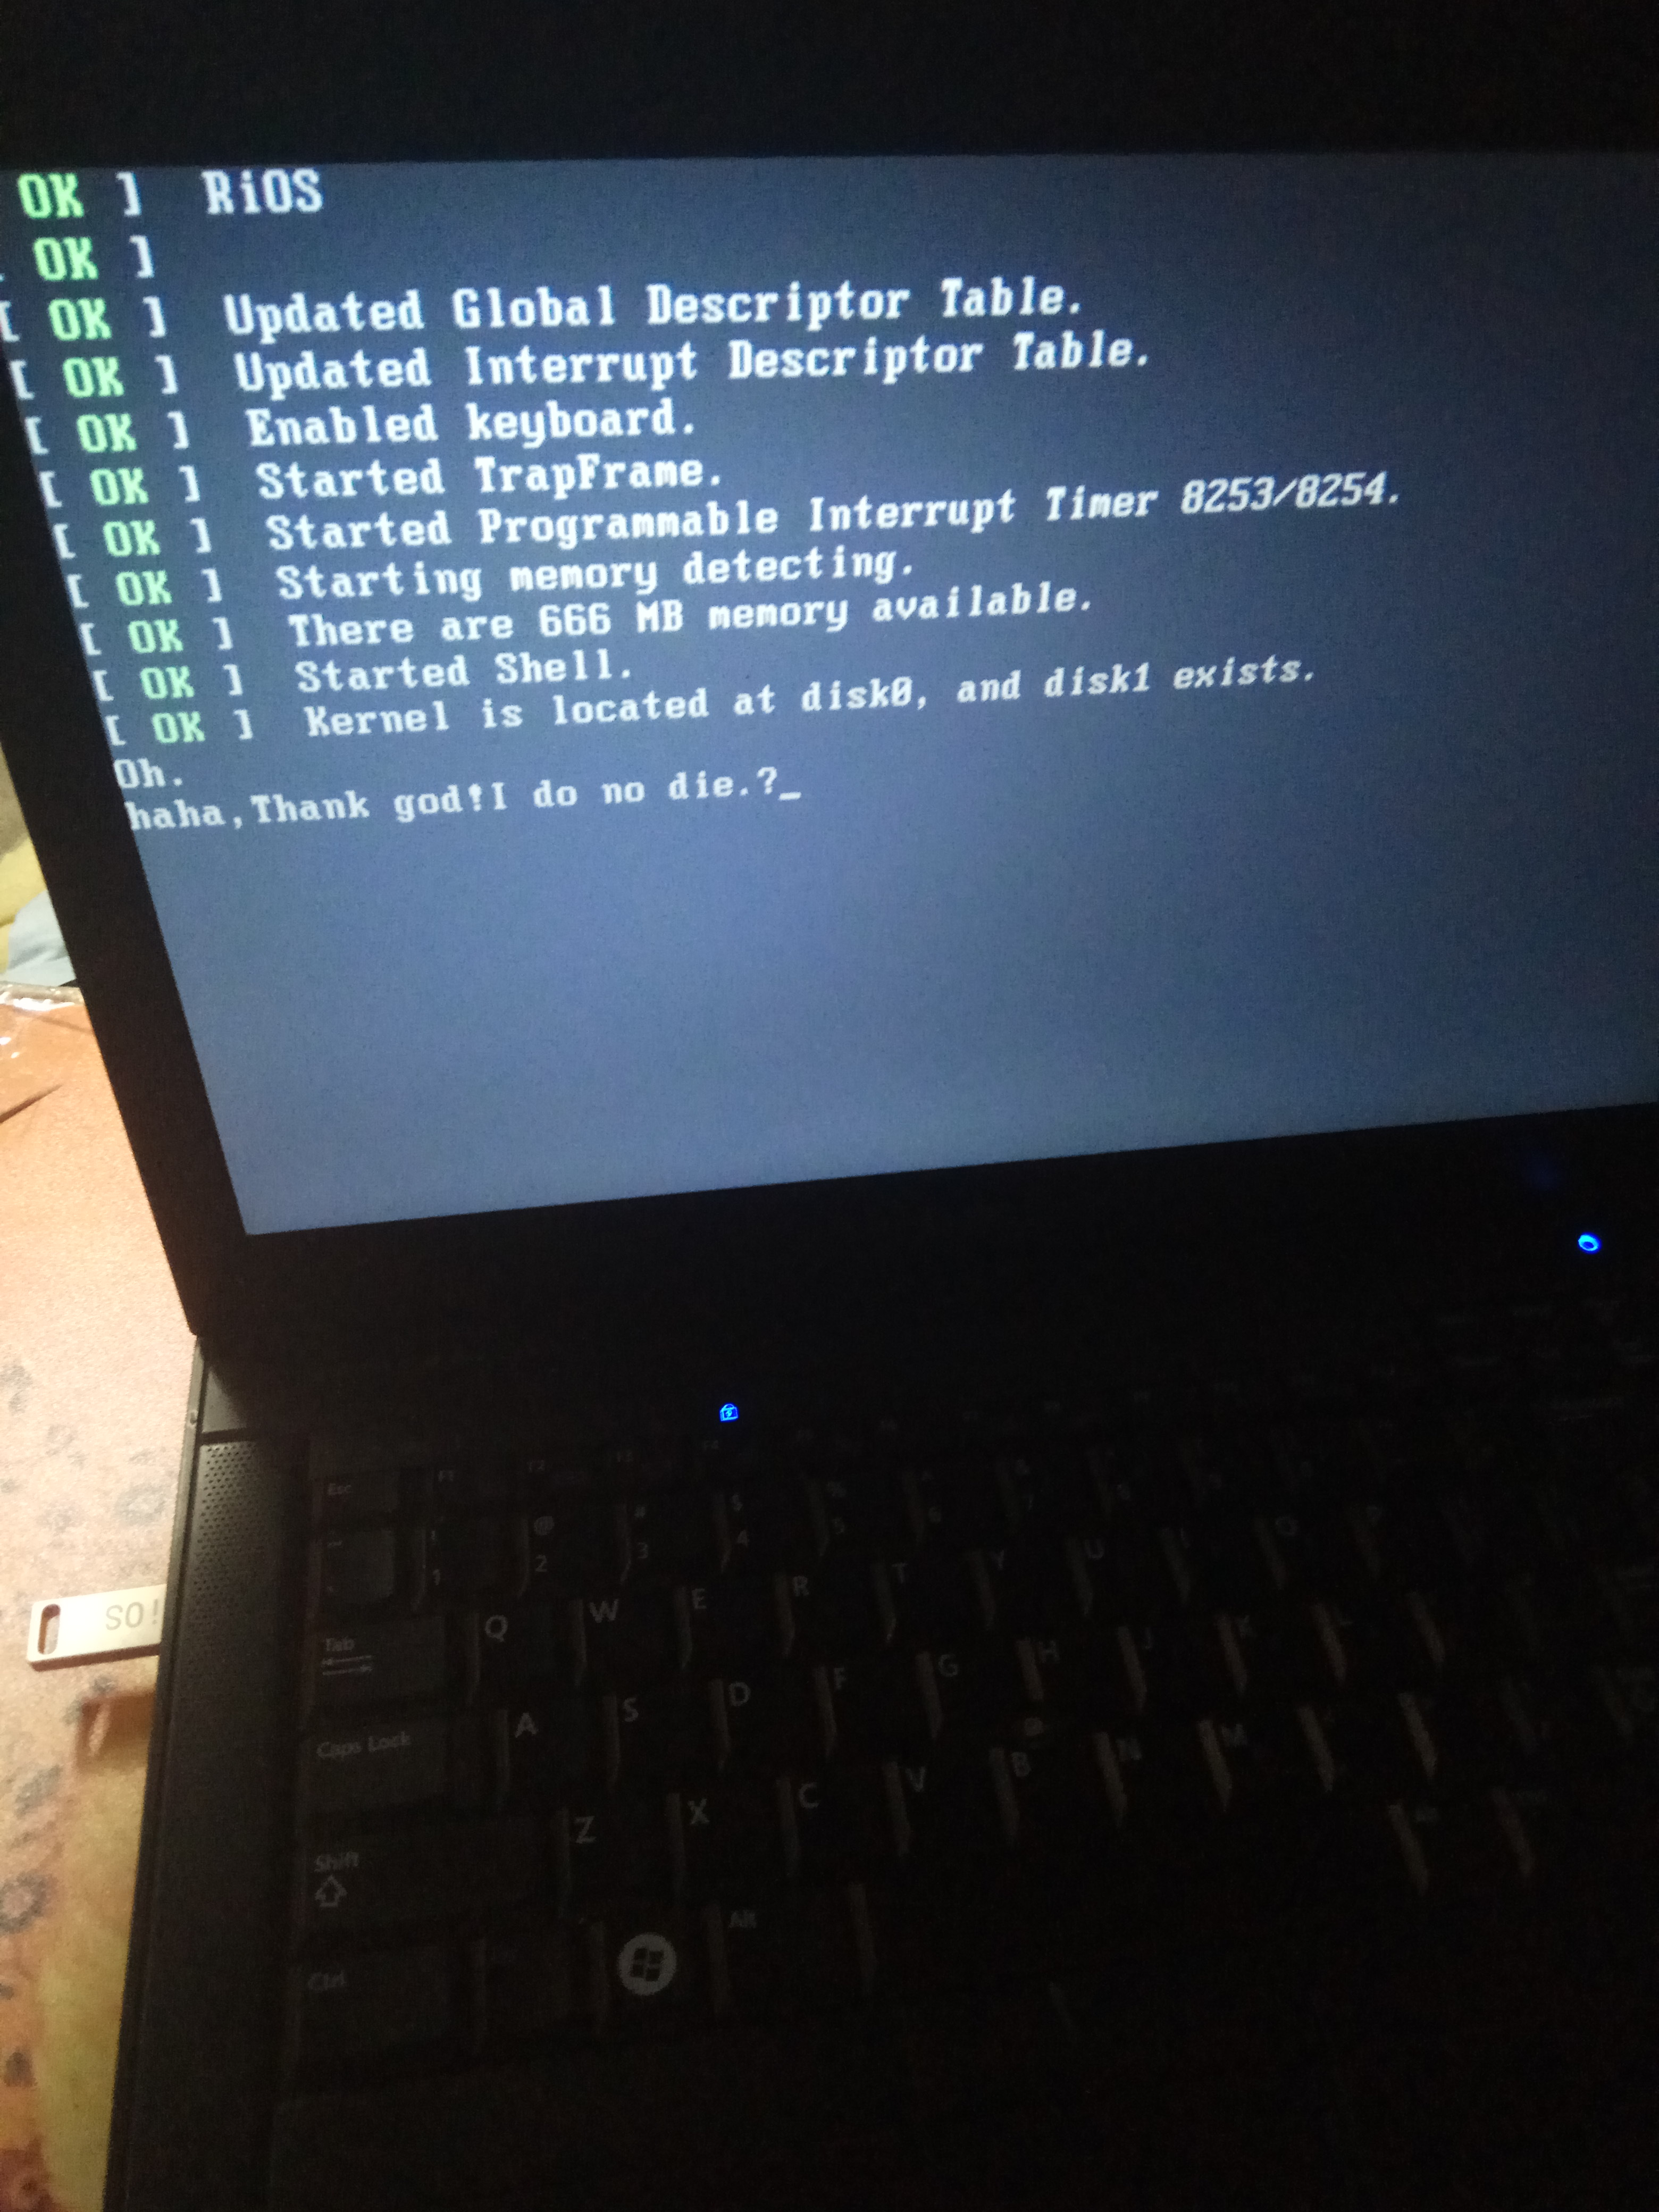
\includegraphics[width=10cm]{pic/assets/testcase/machine}
    \caption{早期裸机测试(非目前最终版本)}	\label{machine}	\end{figure}

\section{利用QEMU模拟器测试}

这里我们开发所用的宿主机操作系统为Ubuntu,笔者用的是Ubuntu17.04,(后来升级到18.04).
请先安装好依赖.
\begin{minted}{shell}
# 之前应该已安装grub2
sudo apt-get install gcc
sudo apt-get install xorriso
# 安装xorriso 才能执行grub-mkrescue
sudo apt-get install qemu
\end{minted}

目前我的机器环境已经配置好,以上是大致回忆的要安装的东西,可能不完整.若还有依赖,请自行安装和配置.
接下来可以进入我的代码文件夹,也可以从github网站上下载.

\begin{minted}{shell}
git clone https://github.com/Twopothead/baby-rios
cd baby-rios
make
\end{minted}

系统测试结果如图~\ref{r1}~所示.

\begin{figure}[!htbp]
    \centering	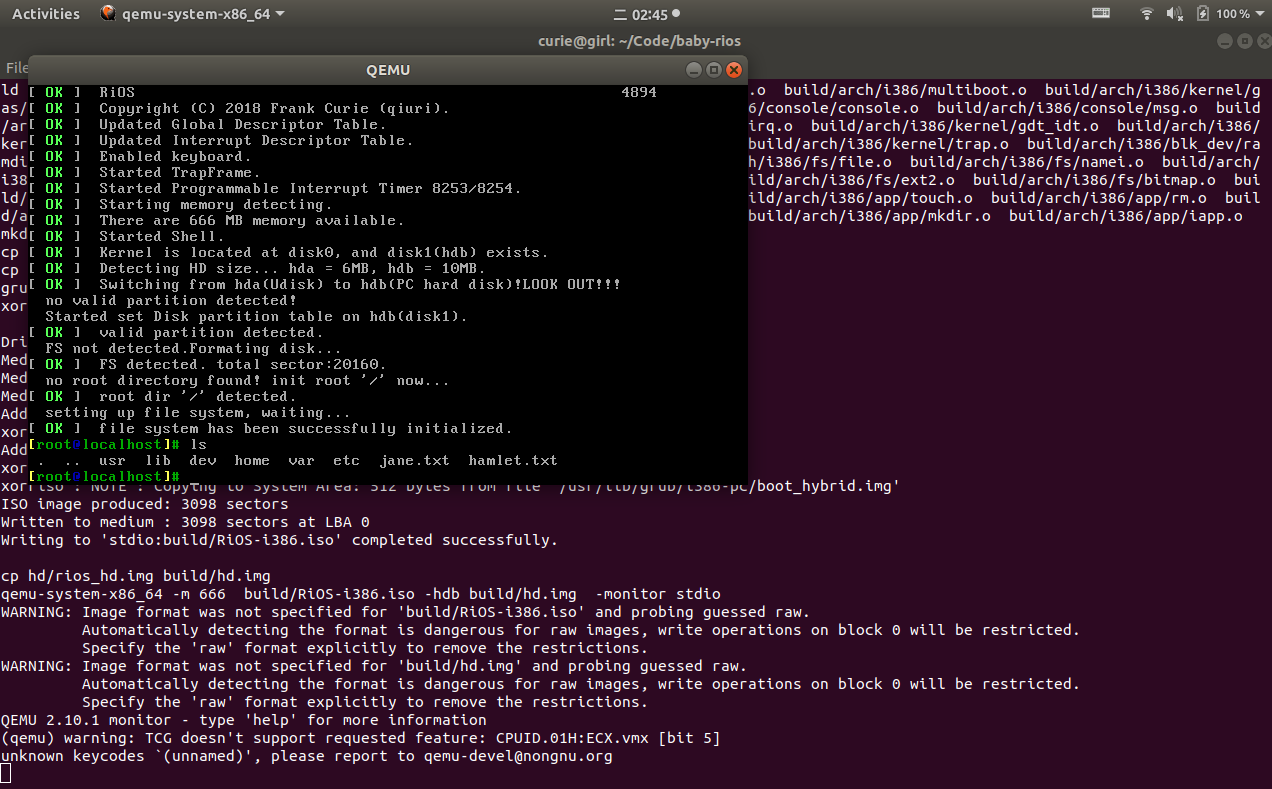
\includegraphics[width=14cm]{pic/assets/testcase/r1}
    \caption{第一次进系统}	\label{r1}	\end{figure}

\begin{minted}{shell}
#这里的命令不是在Ubuntu中运行,而是在qemu虚拟机中使用
ls
cd home
cd qiuri
cd /
cd var
ls 
cd /
cd etc
ls
cd getty
ls
cd /
mkdir dir1/dir2/dir3
ls
cd dir1/dir2/dir3
ls
cd ..
ls
clear
cd /
help
pwd
cd home/qiuri
pwd
info superblock
info disk
info grouping
ls
cd ..
ls
rmdir qiuri
ls
cd ..
ls
rmdir home
ls
cat hamlet.txt
cat jane.txt
ls
rm hamlet.txt
\end{minted}

当然cat jane.txt可能显示过快,看不清楚,系统中还可以使用slowcat jane.txt来显示,
这样可以看清楚了,不过要把一本书从头到尾打印到屏幕,前者要1分钟,后者可能要一下午了.

系统测试结果2如图~\ref{r2}~所示.

\begin{figure}[!htbp]
    \centering	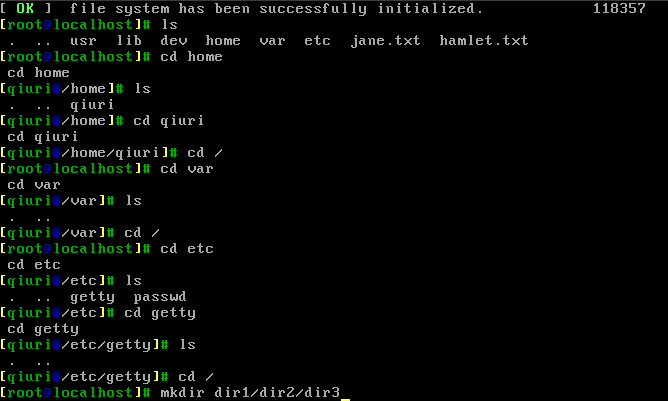
\includegraphics[width=14cm]{pic/assets/testcase/r2}
    \caption{系统测试2}	\label{r2}	\end{figure}

系统测试结果3如图~\ref{r3}~所示.

\begin{figure}[!htbp]
    \centering	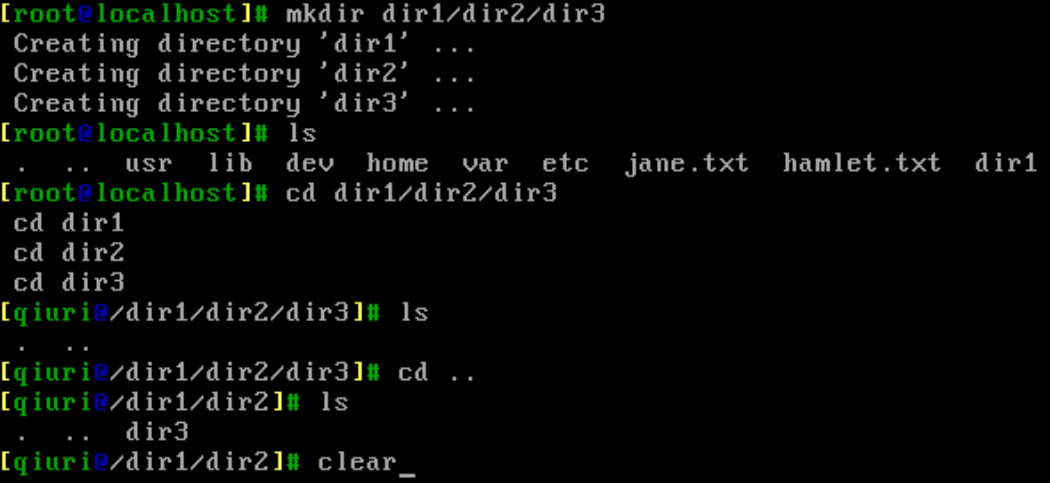
\includegraphics[width=14cm]{pic/assets/testcase/r3}
    \caption{系统测试3}	\label{r3}	\end{figure}

系统测试结果4如图~\ref{r4}~所示.

\begin{figure}[!htbp]
    \centering	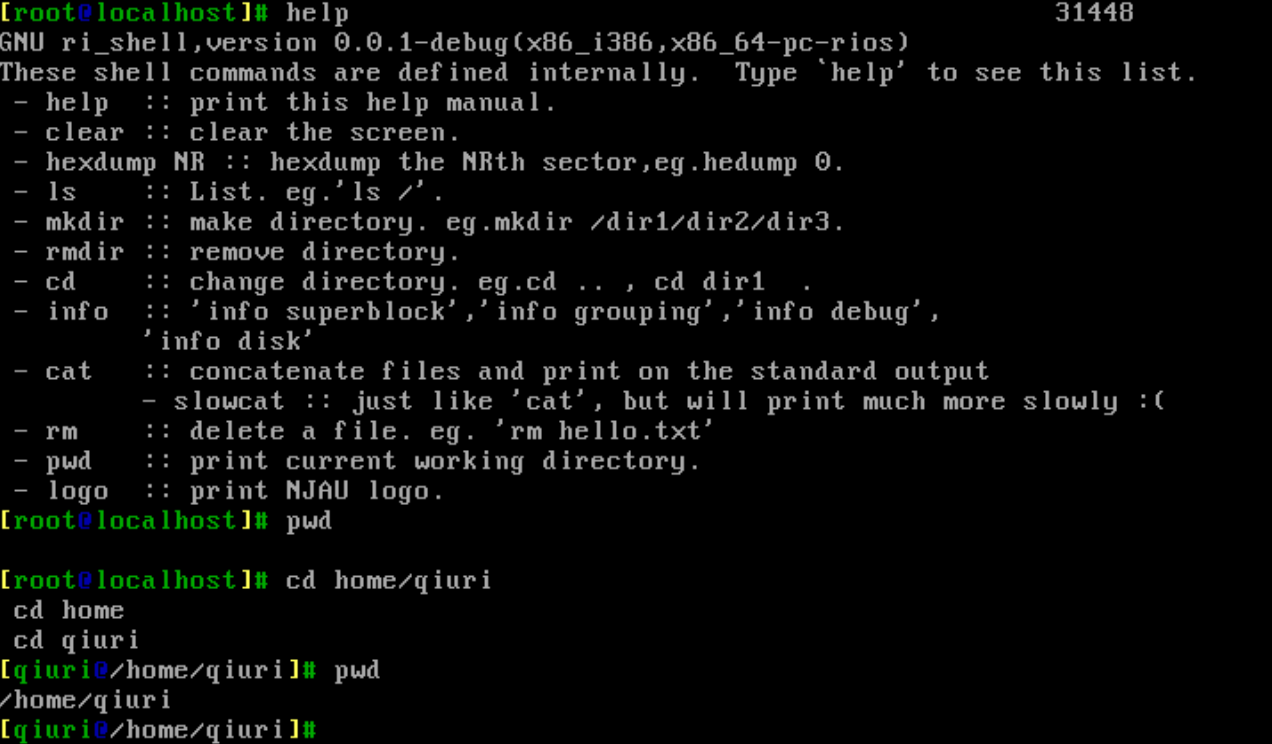
\includegraphics[width=14cm]{pic/assets/testcase/r4}
    \caption{系统测试4}	\label{r4}	\end{figure}

系统测试结果5如图~\ref{r5}~所示.

\begin{figure}[!htbp]
    \centering	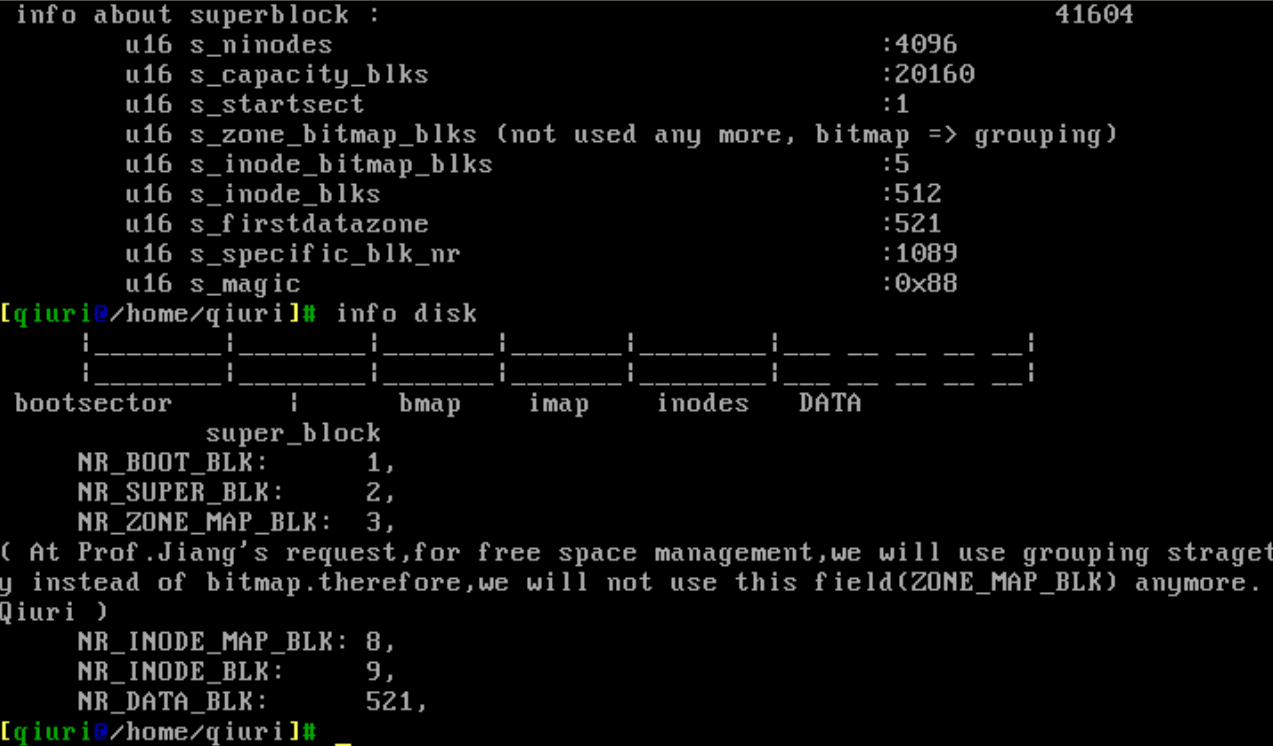
\includegraphics[width=14cm]{pic/assets/testcase/r5}
    \caption{系统测试5}	\label{r5}	\end{figure} 

系统测试结果6如图~\ref{r6}~所示.

\begin{figure}[!htbp]
    \centering	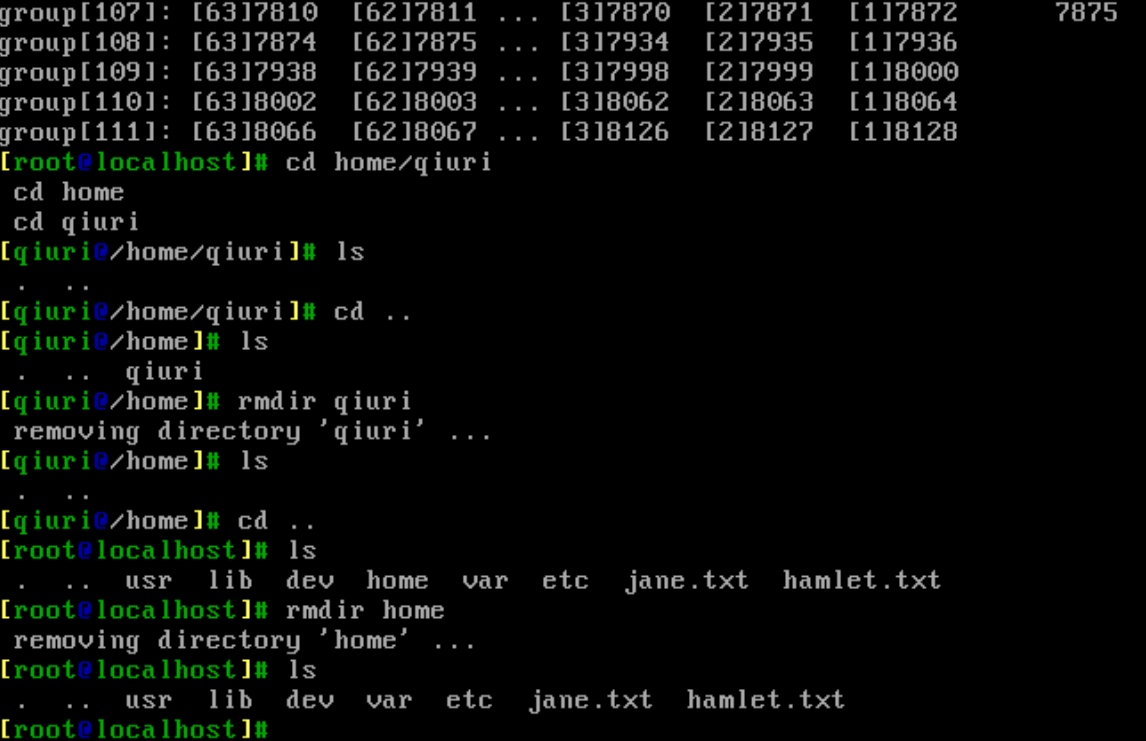
\includegraphics[width=14cm]{pic/assets/testcase/r6}
    \caption{系统测试6}	\label{r6}	\end{figure} 

系统测试结果7如图~\ref{r7}~所示.

\begin{figure}[!htbp]
    \centering	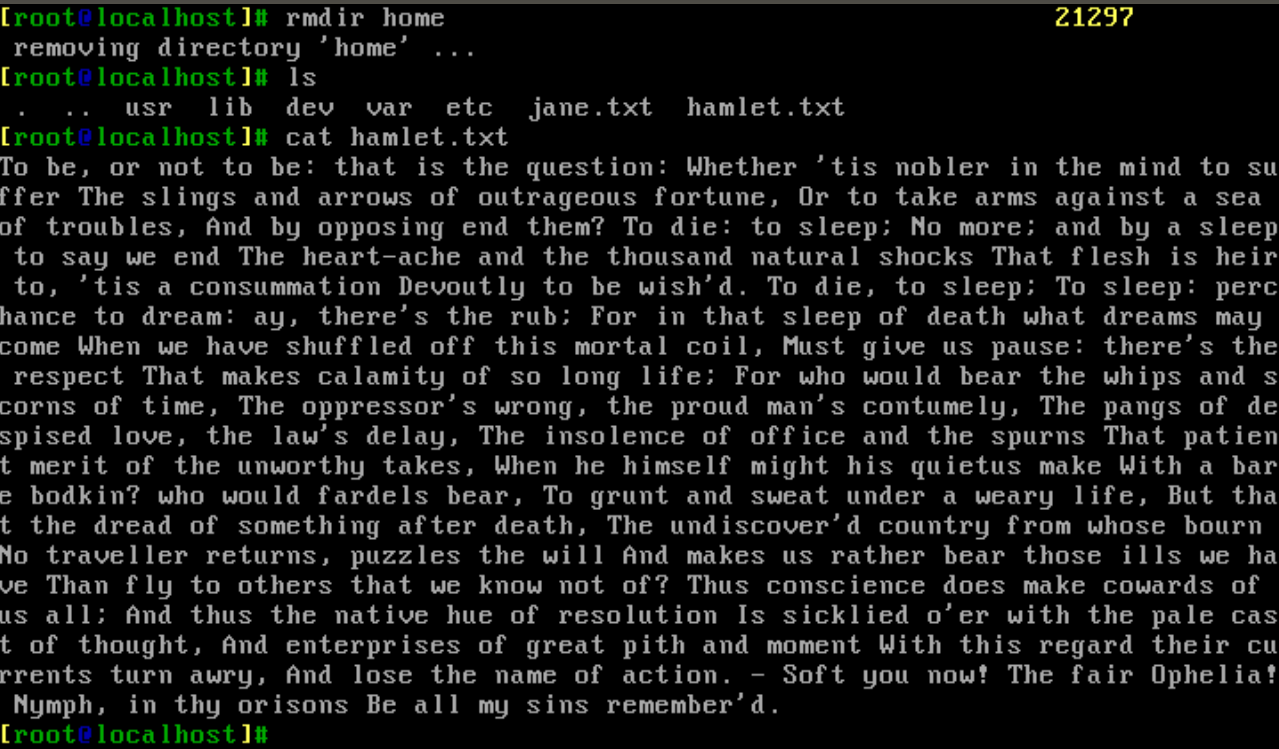
\includegraphics[width=14cm]{pic/assets/testcase/r7}
    \caption{系统测试7}	\label{r7}	\end{figure} 

系统测试结果8如图~\ref{r8}~所示.

\begin{figure}[!htbp]
    \centering	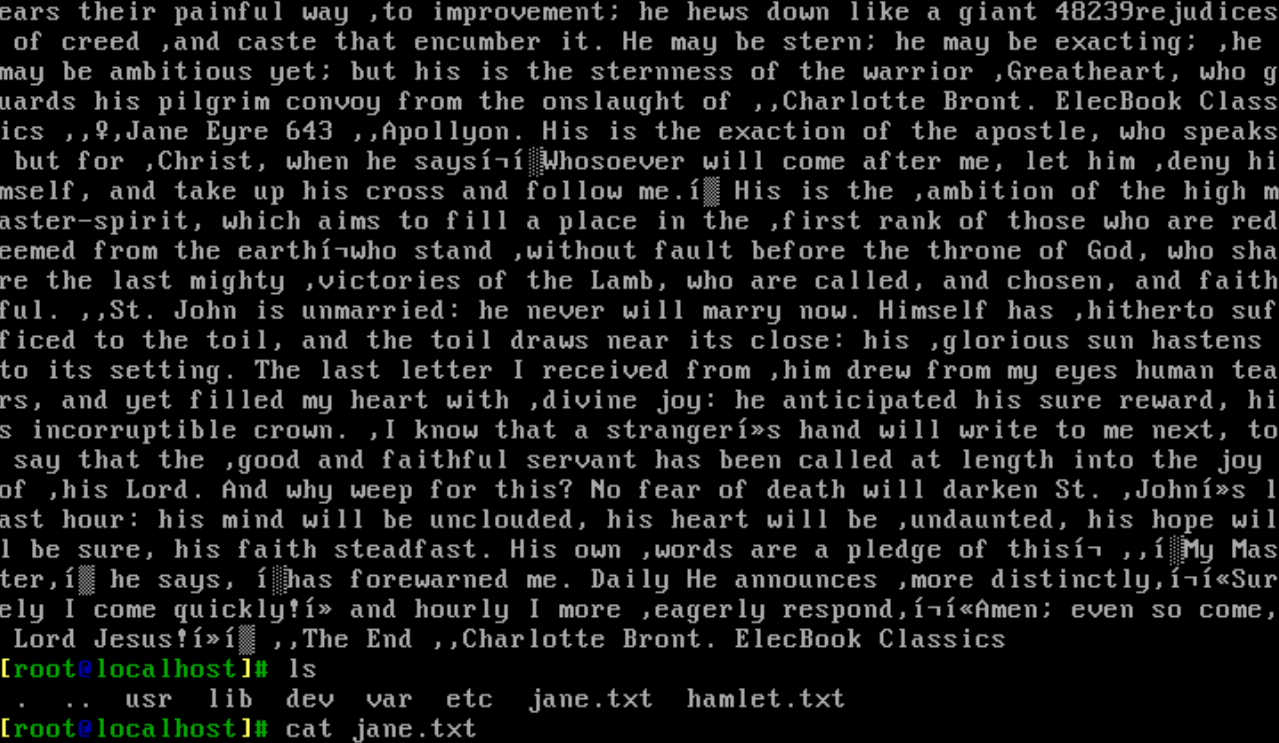
\includegraphics[width=14cm]{pic/assets/testcase/r8}
    \caption{系统测试8}	\label{r8}	\end{figure}    

以上为第一次进系统,我们可以把qemu关掉,再在Ubuntu终端使用make qemu或make run命令
再次进系统.初始化时,系统中有jane,txt(大文件)和hamlet.txt(小文件).
当我们再次进系统时可以看到,因为上次关机时删去了hamlet.txt,故系统中只剩jane.txt.
若上次开机时建立了新目录且没被删掉的话,则下次开机仍能够看到
\begin{minted}{shell}
#这里的命令不是在Ubuntu中运行,而是在qemu虚拟机中使用
ls
cat jane.txt
ls
mkdir dir1/dir2/dir3
\end{minted}

以后要再次进系统可以在Ubuntu终端使用make qemu或make run命令.

如图~\ref{s1}~所示.

\begin{figure}[!htbp]
    \centering	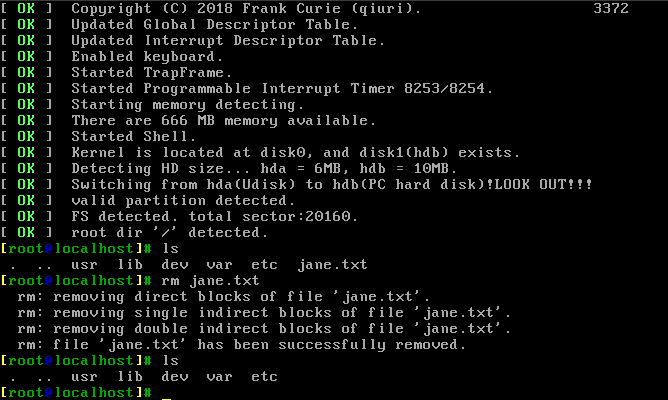
\includegraphics[width=14cm]{pic/assets/testcase/s1}
    \caption{再次进系统测试1}	\label{s1}	\end{figure}  

如果要重新编译,重新建立文件系统.应使用make clean,然后再make.可以自行测试.
    
% \begin{minted}{c}
%     int main() {
%         printf("hello, world");
%         return 0;
%     }
% \end{minted}



% \clearpage